\documentclass[12pt]{article}
\usepackage[usenames]{color} %used for font color
\usepackage{amssymb} %maths
\usepackage{amsmath} %maths
\usepackage[utf8]{inputenc} %useful to type directly diacritic characters
\usepackage[T1]{fontenc}
\usepackage{polski}

% \usepackage{listings}
\usepackage[theme=default-plain]{jlcode} % https://github.com/wg030/jlcode
\usepackage{graphicx}  %grafika

%\usepackage{subcaption} %dwa rysunki obok siebie
%\graphicspath{ {./rysunki/} } %skąd ma pobierać grafikę
%\usepackage{svg} % for graphics in svg, with the first compilation enable: "-shell-escape" to use tools to convert svg
%\usepackage{csvsimple} % to insert csv files 

\usepackage[a4paper, left=3cm, right=3cm, top=1cm, bottom=2cm]{geometry}



\title{Diagram Bifurkacyjny}
\author{Bartosz Zbik}
\date{2024-03-17} %format jest dowolny(może być nawet miesiąc słownie

\begin{document}
\maketitle %tworzy tytuł dokumentu

\noindent Moje rozwiązanie korzysta z faktu, że badane równanie
\begin{equation}
\dot x = r x  + x^3 - x^5
\end{equation}
nie ma rozwiązań uciekających do $\pm \infty$. 

\section{Kod}
\jlinputlisting{solution.jl}



\section{Wizualizacja wyników}
\clearpage

\begin{figure}
\centering
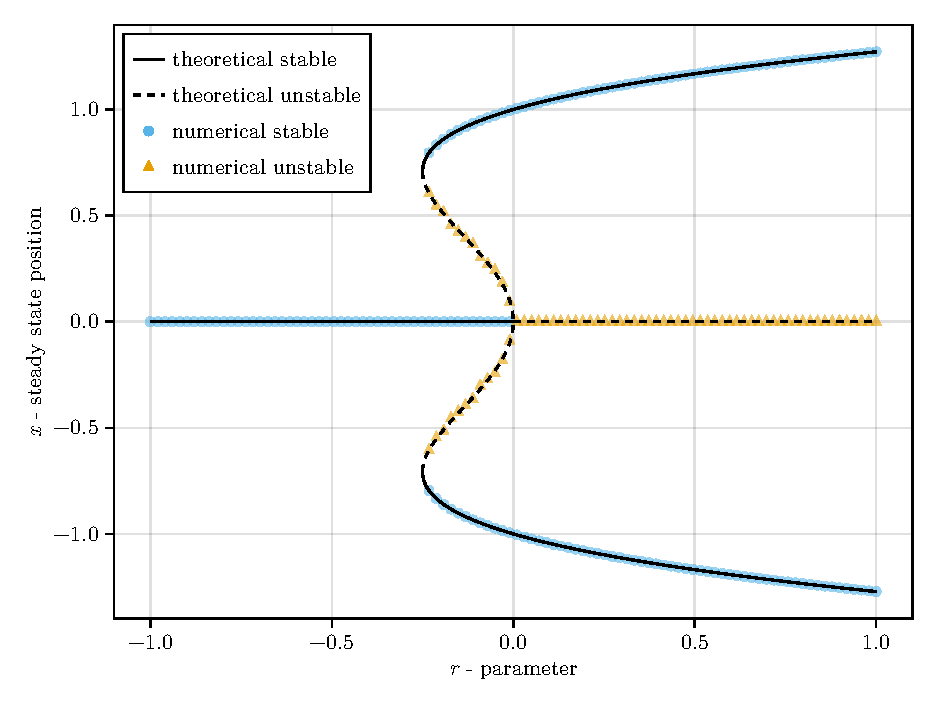
\includegraphics[width=\textwidth]{bifurc-diagram}
\caption{Diagram bifurkacyjny wyznaczony numerycznie (przez rozwiązywanie równania metodą Rungego-Kutty) porównany z analitycznym rozwiązaniem problemu bifurkacji w układzie.}
\end{figure}

\begin{figure}
\centering
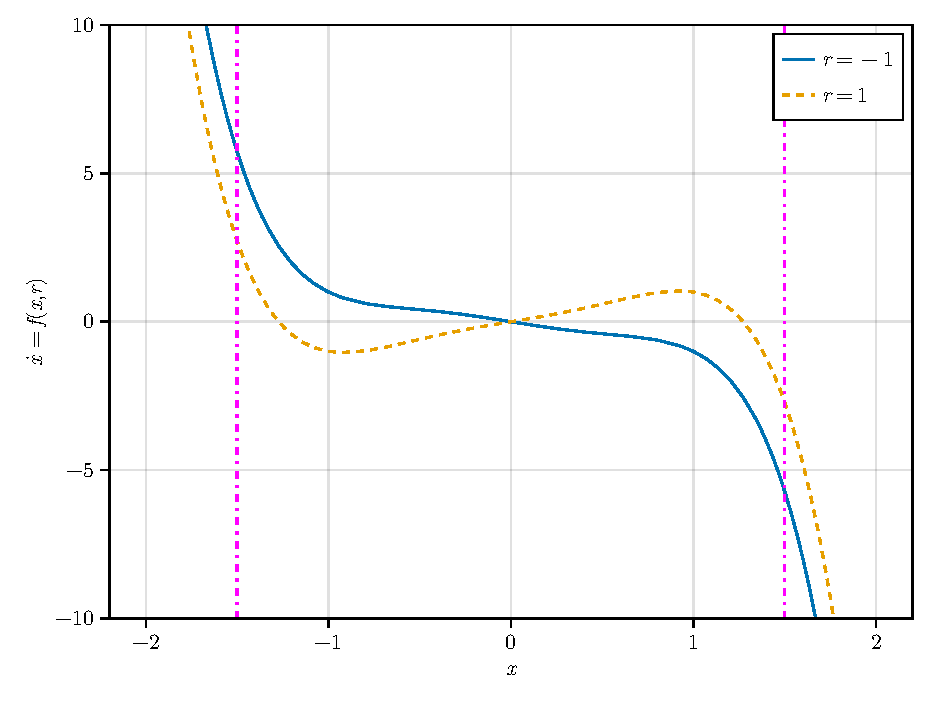
\includegraphics[width=\textwidth]{f-func}
\caption{Zależność $\dot{x}$ od x dla skrajnych badanych wartości $r$.}
\end{figure}



\end{document}